\section{Grundlagen}

\subsection{Problemstellung}

\begin{frame}{\insertsubsection}
  \begin{block}<+->{Zeitreihenreparatur}
    \begin{itemize}
        \item Gegeben:
           \begin{itemize}
                \item Unzuverl�ssige Messung $x = x[1],\dots,x[n]$
                \item Unvollst�ndige, aber daf�r ausschlie�lich korrekte Messung $x^{\text{truth}}$
                \item (Nur bei der Evaluierung: vollst�ndige, korrekte Messung $x^{\text{truth*}}$)
            \end{itemize}
        \item Gesucht:
            \begin{itemize}
                \item Reparatur $y$ mit minimalen RMS-Fehler $\Delta(x^{\text{truth*}}, y)$
                \item $\Delta(x^{\text{truth*}}, y) = \sqrt{\frac{1}{n} \sum_{i=1}^{n} \left(x_i^{\text{truth*}} - y_i\right)^2 }$
            \end{itemize}
    \end{itemize}
  \end{block}
\end{frame}

\subsection{Anomalien}
\begin{frame}[fragile]{\insertsubsection:\ Beispiel\ Eingabe}
\begin{tikzpicture}
\begin{axis}[width=.8\textwidth,
   height=0.8\textheight,
xlabel=Zeit,
ylabel=Datenwert,
legend pos=outer north east,
xmin=0,
ymin=5,
xmax=12
]
\addplot[black, line width=2.0pt, mark size=2.0pt, mark=*]  table{
zeitpunkt wert 
1 6
2 10
3 9.6
4 8.3
5 7.7
6 5.4
7 5.6
8 5.9
9 6.3
10 6.8
11 7.5
12 8.5
};
\addlegendentry{$x$}
\addplot[only marks, red, mark size=5.0pt] table{
zeitpunkt wert 
1 6
2 5.6
3 5.4
6 5.4
12 8.5
};
\addlegendentry{$x^{\text{truth}}$}
% if you have the file, you can do
% \addplot table {datafile.csv};
\end{axis}
\end{tikzpicture}
\end{frame}

\begin{frame}[fragile]{\insertsubsection:\ Beispiel\ Eingabe \& Reperatur}
\begin{tikzpicture}
\begin{axis}[width=.8\textwidth,
   height=0.8\textheight,
xlabel=Zeit,
ylabel=Datenwert,
legend pos=outer north east,
xmin=0,
xmax=12,
ymin=5
]
\addplot[black, line width=2.0pt, mark size=2.0pt, mark=*]  table{
zeitpunkt wert 
1 6
2 10
3 9.6
4 8.3
5 7.7
6 5.4
7 5.6
8 5.9
9 6.3
10 6.8
11 7.5
12 8.5
};
\addlegendentry{$x$}
\addplot[only marks, red, mark size=5.0pt] table{
zeitpunkt wert 
1 6
2 5.6
3 5.4
6 5.4
12 8.5
};
\addlegendentry{$x^{\text{truth}}$}
    \addplot[olive,mark size=5.0pt, mark=x, line width=1.5pt] table{
    zeitpunkt wert 
    1 6
    2 5.6
    3 5.4
    4 5.2
    5 5.4
    6 5.4
    7 5.6
    8 5.9
    9 6.3
    10 6.8
    11 7.5
    12 8.5
    };
    \addlegendentry{$y$}
\end{axis}
\end{tikzpicture}
\end{frame}


\begin{frame}[fragile]{\insertsubsection:\ Beispiel Eingabe \& Reparatur}
\begin{tikzpicture}
\begin{axis}[width=.8\textwidth,
   height=0.8\textheight,
xlabel=Zeit,
ylabel=Datenwert,
ymin=5,
legend pos=outer north east,
xmin=0,
xmax=12
]
\addplot[black, line width=2.0pt, mark size=2.0pt, mark=*]  table{
zeitpunkt wert 
1 6
2 10
3 9.6
4 8.3
5 7.7
6 5.4
7 5.6
8 5.9
9 6.3
10 6.8
11 7.5
12 8.5
};
\addlegendentry{$x$}
\addplot[only marks, red, mark size=5.0pt] table{
zeitpunkt wert 
1 6
2 5.6
3 5.4
6 5.4
12 8.5
};
\addlegendentry{$x^{\text{truth}}$}
    \addplot[olive,mark size=5.0pt, mark=x, line width=1.5pt] table{
    zeitpunkt wert 
    1 6
    2 5.6
    3 5.4
    4 5.2
    5 5.4
    6 5.4
    7 5.6
    8 5.9
    9 6.3
    10 6.8
    11 7.5
    12 8.5
    };
    \addlegendentry{$y$}
   \addplot[blue,mark size=5.0pt, line width=1.5pt] table{
zeitpunkt wert 
1 6
2 5.6
3 5.4
4 5.2
5 5.3
6 5.4
7 5.6
8 5.9
9 6.3
10 6.8
11 7.5
12 8.5
};
\addlegendentry{$x^{\text{truth*}}$}
% if you have the file, you can do
% \addplot table {datafile.csv};
\end{axis}
\end{tikzpicture}
\end{frame}

\begin{frame}{\insertsubsection:\ Beispiel\ Zahlen \& Bewertung}
  \begin{block}<+->{Zeitreihen vom Beispiel}
    \begin{itemize}
    \item $x =                 \{6, 10, 9.6, 8.3, 7.7, 5.4, 5.6, 5.9, 6.3, 6.8, 7.5, 8.5\}$
    \item $x^{\text{truth}} =  \{6, 5.6, 5.4,  \_\_, \_\_,5.4, \_\_,\_\_,\_\_,\_\_,\_\_,8.5\}$
    \item $y =  \{6, 5.6, 5.4, \underline{5.2, {\color{red}5.4}}, 5.4, \underline{5.6, 5.9, 6.3, 6.8, 7.5,} 8.5\}$
    \item $x^{\text{truth*}} =  \{6, 5.6, 5.4,  \underline{5.2, {\color{red}5.3}}, 5.4,\underline{ 5.6, 5.9, 6.3, 6.8, 7.5}, 8.5\}$
    \end{itemize}
  \end{block}
    \begin{block}{Bewertung des Beispiels}
        \[\Delta(x^{\text{truth*}}, y) =\]
        \[
        \sqrt{\frac{1}{12} \left( (6 - 6)^2 + \dots +  (5.3 - 5.4)^2 + \dots + (8.5-8.5)^2\right) } \approx 0.03\]
    \end{block}
\end{frame}


\subsection{Anomalienreparaturen}

\begin{frame}{\insertsubsection}
  \begin{block}<+->{Anomalien}
    \begin{itemize}
      \item Wikipedia: Abweichung von der Regel
      \item Werte $x_i$ mit Abweichung $\tau$ (Bsp. $\tau = 2 \sigma$):\\
          \quad\quad$|x_i-x_i^{\text{truth}}|>\tau$\\
    \end{itemize}
  \end{block}
\end{frame}

\subsection{Reparatur durch Anomalienerkennung}

\begin{frame}{Reparatur durch Anomalienerkennung}
  \begin{block}<+->{Autoregressive Modell $AR(p)$}
    \begin{itemize}
      \item Lineare Regression der letze $p$ Werte:\\
        \[x_t'=\sum_{i=1}^{p}\phi_ix_{t-i}+\epsilon_t\]
      \item Reparatur:
        \[y_t= 
          \begin{cases}
            x_t'& \text{falls} \,\,kein\, Label\, und \,|x_t'-x_t|>\tau\\
            x_t              & \text{sonst}
          \end{cases}\]
    \end{itemize}
  \end{block}
\end{frame}
\begin{frame}{Reparatur durch Anomalienerkennung}
  \begin{block}<+->{Autoregressives exogenes Modell $ARX(p)$}
    \begin{itemize}
      \item Exogenes Variabel $y$\\
      \[y_t'=x_t+\sum_{i=1}^{p}\phi_i(y_{t-i}-x_{t-i})+\epsilon_t\]
      \item $y_t'$ M�gliche Reparatur:
        \[y_t= 
          \begin{cases}
            y_t'& \text{falls} \,\,kein\, Label\, und \,|y_t'-x_t|>\tau\\
            y_t              & \text{sonst}
          \end{cases}\]
      \item 
    \end{itemize}
  \end{block}
\end{frame}

\begin{frame}[fragile]{ARX Reparatur Beispiel}
\begin{columns}
\begin{column}{0.4\textwidth}
ARX(1) mit \\
$p=1$, $\phi=0.5$ und $\tau=0.1$ \\ 
$y_4'=8.3 + 0.5 \cdot (5.4 - 9.6)$ \\ 
$y_4' = 6.2$\\
$|6.2 - 8.3| = 2.1 > 0.1$\\
$y_4=y_4'=6.2$
\end{column}
\begin{column}{0.6\textwidth}  %%<--- here
 \begin{tikzpicture}
\begin{axis}[width=\textwidth,
   height=0.8\textheight,
xlabel=Zeit,
ylabel=Datenwert,
ymin=5,
xmin=0,
xmax=12
]
\addplot[black, line width=2.0pt, mark size=2.0pt, mark=*]  table{
zeitpunkt wert 
1 6
2 10
3 9.6
4 8.3
5 7.7
6 5.4
7 5.6
8 5.9
9 6.3
10 6.8
11 7.5
12 8.5
};
\addlegendentry{$x$}
\addplot[only marks, red, mark size=5.0pt] table{
zeitpunkt wert 
3 5.4
};
\addlegendentry{$x^{\text{truth}}$}
    \addplot[olive,mark size=5.0pt, mark=x, line width=1.5pt] table{
    zeitpunkt wert 
    4 6.2 
    };
    \addlegendentry{$y$}
   \addplot[blue,mark size=5.0pt, line width=1.5pt] table{
zeitpunkt wert 
1 6
2 5.6
3 5.4
4 5.2
5 5.3
6 5.4
7 5.6
8 5.9
9 6.3
10 6.8
11 7.5
12 8.5
};
\addlegendentry{$x^{\text{truth*}}$}
% if you have the file, you can do
% \addplot table {datafile.csv};
\end{axis}
\end{tikzpicture}
\end{column}
\end{columns}
\end{frame}
\begin{frame}{Andere Reparaturen}
  \begin{block}<+->{Gleitender Mittelwert}
    \begin{itemize}
      \item 
      \[
    y_j = \frac{1}{k}\sum_{i=1}^{k}x_{j-i} \quad j \in \{k,..,n\}
      \] 
    \end{itemize}
  \end{block}
  \begin{block}<+->{Exponentiell Gewichteten Gleitender Mittelwert (EWMA)}
    \begin{itemize}
      \item 
  \[
    v_j = \sum_{i=0}^{n}(\beta-1)\beta^{i}x_{j-i}\quad j \in \{k,..,n\}
  \]
  as
  \[
   v_j = \beta v_{j-1} + (1-\beta)x_j \quad mit\,\, V_0=0
  \]
    \end{itemize}
  \end{block}
  \begin{block}<+->{SCREEN}
    \begin{itemize}
      \item 
    \end{itemize}
  \end{block}
\end{frame}


